% TPCU 碩士學位論文 LaTex 樣板
% 使用 utf-8 編碼
% v0.5 (Jun. 30, 2012)
% by Peter

\documentclass[a4paper,12pt]{report}


% 引用必要的套件
\usepackage{tpcu}
\usepackage[english]{babel}
\usepackage{blindtext}

%\usepackage{chap_last}

\usepackage{xcolor,tikz}
%\usepackage[usenames,dvipsnames,pdftex]{xcolor}
%\def\pgfsysdriver{pgfsys-dvipdfmx.def}
%\usepackage{tikz,ifthen}

\newcommand{\newchapter}[1]{%
    \chapter{#1}
%   \pagestyle{fancy}
    \thispagestyle{fancy}
%   \fancyhead[LO,RE]{\slshape \leftmark}
    \fancyhead[LE,RO]{\slshape \leftmark}
    \fancyfoot[C]{\thepage}
%   \fontsize{16}{20}\selectfont
}
%\usepackage{CJKnumb} %%% ZZZ %%% for Chinese numbering capability
%\usepackage[nospace]{cite}  % for smart citation

%%%%%%%%%%%%%%%%%%%%%%%%%%%%%
%  end of preamble
%%%%%%%%%%%%%%%%%%%%%%%%%%%%%

% define the title
\begin{document}

\large 
\fontsize{14}{20}\selectfont
%
% 使用 utf-8 編碼
% v2.0 (Apr. 5, 2009)
% do not change the content of this file
% unless the thesis layout rule is changed
% 無須修改本檔內容,除非校方修改了
% 封面、書名頁、中文摘要、英文摘要、誌謝、目錄、表目錄、圖目錄、符號說明
% 等頁之格式

% make the line spacing in effect
\renewcommand{\baselinestretch}{\mybaselinestretch}
\large % it needs a font size changing command to be effective

% default variables definitions
% 此處只是預設值,不需更改此處
% 請更改 my_names.tex 內容
\newcommand\cTitle{論文題目}
\newcommand\eTitle{MY THESIS TITLE}
\newcommand\myCname{王鐵雄}
\newcommand\myEname{Aron Wang}
\newcommand\advisorCnameA{南宮明博士}
\newcommand\advisorEnameA{Dr.~Ming Nangong}
\newcommand\advisorCnameB{李斯坦博士}
\newcommand\advisorEnameB{Dr.~Stein Lee}
\newcommand\advisorCnameC{徐 石博士}
\newcommand\advisorEnameC{Dr.~Sean~Hsu}
\newcommand\univCname{臺北城市大學}
\newcommand\univEname{Taipei Chengshih University of Science and Technology}
\newcommand\deptCname{電子商務研究所}
\newcommand\fulldeptEname{Institute of E-Commerce}
\newcommand\deptEname{Institute of E-Commerce}
\newcommand\collEname{College of Business and Management}
\newcommand\degreeCname{碩士}
\newcommand\degreeEname{Master}
\newcommand\cYear{九十四}
\newcommand\cMonth{六}
\newcommand\cDay{}
\newcommand\eYear{2006}
\newcommand\eMonth{June}
\newcommand\eDay{}
\newcommand\ePlace{Taipei, Taiwan}


 % user's names; to replace those default variable definitions
% 使用 utf-8 編碼
% v2.0 (Apr. 5, 2009)
% 填入你的論文題目、姓名等資料
% 如果題目內有必須以數學模式表示的符號,請用 \mbox{} 包住數學模式,如下範例
% 如果中文名字是單名,與姓氏之間建議以全形空白填入,如下範例
% 英文名字中的稱謂,如 Prof. 以及 Dr.,其句點之後請以不斷行空白~代替一般空白,如下範例
% 如果你的指導教授沒有如預設的三位這麼多,則請把相對應的多餘教授的中文、英文名
%    的定義以空的大括號表示
%    如,\renewcommand\advisorCnameB{}
%          \renewcommand\advisorEnameB{}
%          \renewcommand\advisorCnameC{}
%          \renewcommand\advisorEnameC{}

% 論文題目 (中文)
\renewcommand\cTitle{%
品牌聲望及品牌知覺對消費決策為與消費者滿意度影響之研究-以飾品業 La Jolla公司為例(論文初稿)}

% 論文題目 (英文)
\renewcommand\eTitle{
A study of the Influences of Brand perception and Brand Reputation on consumer decision making and Consumer satisfaction – A case study of La Jolla jewelry company}

% 我的姓名 (中文)
\renewcommand\myCname{盧建璋}

% 我的姓名 (英文)
\renewcommand\myEname{jian-Jhang Lu}

% 指導教授A的姓名 (中文)
\renewcommand\advisorCnameA{林慶昌 博士}

% 指導教授A的姓名 (英文)
\renewcommand\advisorEnameA{Dr.~Ching-Chang Lin}

% 指導教授B的姓名 (中文)
\renewcommand\advisorCnameB{}

% 指導教授B的姓名 (英文)
\renewcommand\advisorEnameB{}

% 指導教授C的姓名 (中文)
\renewcommand\advisorCnameC{}

% 指導教授C的姓名 (英文)
\renewcommand\advisorEnameC{}

% 校名 (中文)
\renewcommand\univCname{臺北城市科技大學}

% 校名 (英文)
\renewcommand\univEname{Taipei Chengshih University of Science and Technology}

% 系所名 (中文)
\renewcommand\deptCname{電子商務研究所}

% 系所全名 (英文)
\renewcommand\fulldeptEname{Institute of E-Commerce}

% 系所短名 (英文, 用於書名頁學位名領域)
\renewcommand\deptEname{Institute of E-Commerce}

% 學院英文名 (如無,則以空的大括號表示)
\renewcommand\collEname{College of Business and Management}

% 學位名 (中文)
\renewcommand\degreeCname{碩士}

% 學位名 (英文)
\renewcommand\degreeEname{Master}

% 口試年份 (中文、民國)
\renewcommand\cYear{一百零二}

% 口試月份 (中文)
\renewcommand\cMonth{六}

% 口試日 (中文)
\renewcommand\cDay{二十六}

% 口試年份 (阿拉伯數字、西元)
\renewcommand\eYear{2013}

% 口試月份 (英文)
\renewcommand\eMonth{June}

% 口試日 (英文)
\renewcommand\eDay{26}


% 學校所在地 (英文)
\renewcommand\ePlace{Taipei, Taiwan}

%畢業級別;用於書背列印;若無此需要可忽略
\newcommand\GraduationClass{100}

%%%%%%%%%%%%%%%%%%%%%%


% 使用 hyperref 在 pdf 簡介欄裡填入相關資料
\ifx\hypersetup\undefined
	\relax  % do nothing
\else
	\hypersetup{
	pdftitle=\cTitle,
	pdfauthor=\myCname}
\fi
	

\newcommand\itsempty{}
%%%%%%%%%%%%%%%%%%%%%%%%%%%%%%%
%       TPCU cover 封面
%%%%%%%%%%%%%%%%%%%%%%%%%%%%%%%
%
\begin{titlepage}
% no page number
% next page will be page 1

% aligned to the center of the page
\begin{center}
% font size (relative to 12 pt):
% \large (14pt) < \Large (18pt) < \LARGE (20pt) < \huge (24pt)< \Huge (24 pt)
%
\makebox[6cm][s]{\Huge{\univCname}}\\  %顯示中文校名
\vspace{1.5cm}
\makebox[12cm][s]{\Huge{\deptCname}}\\ %顯示中文系所名
\vspace{1.5cm}
\makebox[6cm][s]{\Huge{\degreeCname 論文}}\\ %顯示論文種類 (中文)
% 初稿論文
\vspace{1.5cm}\makebox[2cm][s]{\Large{(初稿)}}\\ %顯示論文種類 (中文)
\vspace{3cm}
%
% Set the line spacing to single for the titles (to compress the lines)
\renewcommand{\baselinestretch}{1}   %行距 1 倍
%\large % it needs a font size changing command to be effective
%\Large{\cTitle}\\  % 中文題目
\fontsize{20}{22}\selectfont{\cTitle} \\
%
\vspace{1cm}
%
%\Large{\eTitle}\\ %英文題目
\fontsize{20}{22}\selectfont{\eTitle} \\

\vspace{4cm}
% \makebox is a text box with specified width;
% option s: stretch
% use \makebox to make sure
% 「研究生:」 與「指導教授:」occupy the same width
\hspace{4.5cm} \makebox[3cm][s]{\Large{研 究 生:}}
\Large{\myCname}  % 顯示作者中文名
\hfill \makebox[1cm][s]{}\\
%
\vspace{1cm}
\hspace{4.5cm} \makebox[3cm][s]{\Large{指導教授:}}
\Large{\advisorCnameA}  %顯示指導教授A中文名
\hfill \makebox[1cm][s]{}\\
%
% 判斷是否有共同指導的教授 B
\ifx \advisorCnameB  \itsempty
\relax % 沒有 B 教授,所以不佔版面,不印任何空白
\else
% 共同指導的教授 B
\hspace{4.5cm} \makebox[3cm][s]{}
\Large{\advisorCnameB}  %顯示指導教授B中文名
\hfill \makebox[1cm][s]{}\\
\fi
%
% 判斷是否有共同指導的教授 C
\ifx \advisorCnameC  \itsempty
\relax % 沒有 C 教授,所以不佔版面,不印任何空白
\else
% 共同指導的教授 C
\hspace{4.5cm} \makebox[3cm][s]{}
\Large{\advisorCnameC}  %顯示指導教授C中文名
\hfill \makebox[1cm][s]{}\\
\fi
%
\vfill
\makebox[10cm][s]{\Large{中華民國\cYear 年\cMonth 月}}%
%
\end{center}
% Resume the line spacing to the desired setting
\renewcommand{\baselinestretch}{\mybaselinestretch}   %恢復原設定
% it needs a font size changing command to be effective
% restore the font size to normal
\normalsize
\end{titlepage}
%%%%%%%%%%%%%%

%% 從摘要到本文之前的部份以小寫羅馬數字印頁碼
% 但是從「書名頁」(但不印頁碼) 就開始計算
\setcounter{page}{1}
\pagenumbering{roman}
%%%%%%%%%%%%%%%%%%%%%%%%%%%%%%%
%       書名頁
%%%%%%%%%%%%%%%%%%%%%%%%%%%%%%%
%
\newpage

% 判斷是否要浮水印?
\ifx\mywatermark\undefined
  \thispagestyle{empty}  % 無頁碼、無 header (無浮水印)
\else
  \thispagestyle{EmptyWaterMarkPage} % 無頁碼、有浮水印
\fi

%no page number
% create an entry in table of contents for 書名頁
\phantomsection % for hyperref to register this
\addcontentsline{toc}{chapter}{\nameInnerCover}


% aligned to the center of the page
\begin{center}
% font size (relative to 12 pt):
% \large (14pt) < \Large (18pt) < \LARGE (20pt) < \huge (24pt)< \Huge (24 pt)
% Set the line spacing to single for the titles (to compress the lines)
\renewcommand{\baselinestretch}{1}   %行距 1 倍
% it needs a font size changing command to be effective
%中文題目
\Large{\cTitle}\\ %%%%%
\vspace{1cm}
% 英文題目
\Large{\eTitle}\\ %%%%%
%\vspace{1cm}
\vfill
% \makebox is a text box with specified width;
% option s: stretch
% use \makebox to make sure
% 「研究生:」 與「指導教授:」occupy the same width
\makebox[3cm][s]{\large{研 究 生:}}
\makebox[3cm][l]{\large{\myCname}} %%%%%
\hfill
\makebox[2cm][s]{\large{Student: }}
\makebox[5cm][l]{\large{\myEname}}\\ %%%%%
%
%\vspace{1cm}
%
\makebox[3cm][s]{\large{指導教授:}}
\makebox[3cm][l]{\large{\advisorCnameA}} %%%%%
\hfill
\makebox[2cm][s]{\large{Advisor: }}
\makebox[5cm][l]{\large{\advisorEnameA}}\\ %%%%%
%
% 判斷是否有共同指導的教授 B
\ifx \advisorCnameB  \itsempty
\relax % 沒有 B 教授,所以不佔版面,不印任何空白
\else
%共同指導的教授B
\makebox[3cm][s]{}
\makebox[3cm][l]{\large{\advisorCnameB}} %%%%%
\hfill
\makebox[2cm][s]{}
\makebox[5cm][l]{\large{\advisorEnameB}}\\ %%%%%
\fi
%
% 判斷是否有共同指導的教授 C
\ifx \advisorCnameC  \itsempty
\relax % 沒有 C 教授,所以不佔版面,不印任何空白
\else
%共同指導的教授C
\makebox[3cm][s]{}
\makebox[3cm][l]{\large{\advisorCnameC}} %%%%%
\hfill
\makebox[2cm][s]{}
\makebox[5cm][l]{\large{\advisorEnameC}}\\ %%%%%
\fi
%
% Resume the line spacing to the desired setting
\renewcommand{\baselinestretch}{\mybaselinestretch}   %恢復原設定
\large %it needs a font size changing command to be effective
%
\vfill
\makebox[4cm][s]{\large{\univCname}}\\% 校名
\makebox[6cm][s]{\large{\deptCname}}\\% 系所名
\makebox[3cm][s]{\large{\degreeCname 論文}}\\% 學位名
%
%\vspace{1cm}
\vfill
\large{A Thesis}\\%
\large{Submitted to }%
%
\large{\fulldeptEname}\\%系所全名 (英文)
%
%
\ifx \collEname  \itsempty
\relax % 沒有學院名 (英文),所以不佔版面,不印任何空白
\else
% 有學院名 (英文)
\large{\collEname}\\% 學院名 (英文)
\fi
%
\large{\univEname}\\%校名 (英文)
%
\large{in Partial Fulfillment of the Requirements}\\
%
\large{for the Degree of}\\
%
\large{\degreeEname}\\%學位名(英文)
%
\large{in}\\
%
\large{\deptEname}\\%系所短名(英文;表明學位領域)
%
\large{\eMonth\ \eYear}\\%月、年 (英文)
%
\large{\ePlace}% 學校所在地 (英文)
\vfill
\makebox[10cm][s]{\Large{中華民國\cYear 年\cMonth 月}}
%\large{中華民國}%
%\large{\cYear}% %%%%%
%\large{年}%
%\large{\cMonth}% %%%%%
%\large{月}\\
\end{center}
% restore the font size to normal
\normalsize
\clearpage
%%%%%%%%%%%%%%%%%%%%%%%%%%%%%%%
%       論文口試委員審定書 (計頁碼,但不印頁碼)
%%%%%%%%%%%%%%%%%%%%%%%%%%%%%%%
%
% insert the printed standard form when the thesis is ready to bind
% 在口試完成後,再將已簽名的審定書放入以便裝訂
% create an entry in table of contents for 審定書
% 目前送出空白頁
\newpage%
%\begin{CJK}{UTF8}{nkai}
\thispagestyle{EmptyWaterMarkPage}  % 無 header,但在浮水印模式下會有浮水印
\phantomsection % for hyperref to register this
\addcontentsline{toc}{chapter}{\nameCommitteeForm}%

\begin{center}
\fontsize{24}{36}\selectfont 碩士學位論文考試委員會審定書\\
\vspace{0.5cm}
\end{center}

\vspace{0.5cm}

%\parbox[s]
%{\cTitle} \\
%{\eTitle} \\

\fontsize{20}{22}\selectfont
本校 \underline{\deptCname} \underline{\myCname}  君\\
所提論文 \uline{\cTitle} \\
%本校 \underline{\deptCname} \underline{\myCname}  君,所提論文 \\
%\fontsize{18}{22}\selectfont\cTitle \\
%\fontsize{20}{22}\selectfont
經本委員會審定通過,合於碩士資格,特此證明。 \\

%\vspace{0.1cm}
\fontsize{20}{16}\selectfont
\begin{tabular}{rp{0.9\textwidth}}
學位考試委員會 \\ & \\
委~員~:
	& \rule{0.6\textwidth}{1pt} \\
	& \\
	& \rule{0.6\textwidth}{1pt} \\
	& \\
	& \rule{0.6\textwidth}{1pt} \\
	& \\
	& \rule{0.6\textwidth}{1pt} \\
	& \\
指~導~教~授~: & \rule{0.6\textwidth}{1pt} \\
	& \\
所~長~: & \rule{0.6\textwidth}{1pt}
\end{tabular}

%\vfill
\vspace{1cm}
\begin{center}
\makebox[10cm][s]{\Large{中華民國\cYear 年\cMonth 月\cDay 日}}
\end{center}
%\large{中華民國}
%\large{\cYear}% %%%%%
%\large{年}
%\large{\cMonth}% %%%%%
%\large{月}
%\large{\cDay}% %%%%%
%\large{日}\\

%\end{CJK}
\clearpage
\normalsize


%%%%%%%%%%%%%%%%%%%%%%%%%%%%%%%
%       論文口試委員審定書 (計頁碼,但不印頁碼)
%%%%%%%%%%%%%%%%%%%%%%%%%%%%%%%
%
% insert the printed standard form when the thesis is ready to bind
% 在口試完成後,再將已簽名的審定書放入以便裝訂
% create an entry in table of contents for 審定書
% 目前送出空白頁
%%\newpage%
%%{\thispagestyle{empty}%
%%\phantomsection % for hyperref to register this
%%\addcontentsline{toc}{chapter}{\nameCommitteeForm}%
%%\mbox{}\clearpage}

%%%%%%%%%%%%%%%%%%%%%%%%%%%%%%%
%       授權書 (計頁碼,但不印頁碼)
%%%%%%%%%%%%%%%%%%%%%%%%%%%%%%%
%
% insert the printed standard form when the thesis is ready to bind
% 在口試完成後,再將已簽名的授權書放入以便裝訂
% create an entry in table of contents for 授權書
% 目前送出空白頁
\newpage%

%\vspace{3cm}
此頁為「論文授權書」,計頁碼,但不印頁碼,

\vspace{3cm}
在口試完成後,再將已簽名的授權書之後,替換本頁以便裝訂。
{\thispagestyle{empty}%
\phantomsection % for hyperref to register this
\addcontentsline{toc}{chapter}{\nameCopyrightForm}%
\mbox{}\clearpage}

%%%%%%%%%%%%%%%%%%%%%%%%%%%%%%%
%       中文摘要
%%%%%%%%%%%%%%%%%%%%%%%%%%%%%%%
%
\newpage
\thispagestyle{plain}  % 無 header,但在浮水印模式下會有浮水印
% create an entry in table of contents for 中文摘要
\phantomsection % for hyperref to register this
\addcontentsline{toc}{chapter}{\nameCabstract}

% aligned to the center of the page
\begin{center}
% font size (relative to 12 pt):
% \large (14pt) < \Large (18pt) < \LARGE (20pt) < \huge (24pt)< \Huge (24 pt)
% Set the line spacing to single for the names (to compress the lines)
\renewcommand{\baselinestretch}{1}   %行距 1 倍
% it needs a font size changing command to be effective
\large{\cTitle}\\  %中文題目
\vspace{0.83cm}
% \makebox is a text box with specified width;
% option s: stretch
% use \makebox to make sure
% each text field occupies the same width
\makebox[1.5cm][s]{\large{學生:}}
\makebox[3cm][l]{\large{\myCname}} %學生中文姓名
\hfill
%
\makebox[3cm][s]{\large{指導教授:}}
\makebox[3cm][l]{\large{\advisorCnameA}} \\ %教授A中文姓名
%
% 判斷是否有共同指導的教授 B
\ifx \advisorCnameB  \itsempty
\relax % 沒有 B 教授,所以不佔版面,不印任何空白
\else
%共同指導的教授B
\makebox[1.5cm][s]{}
\makebox[3cm][l]{} %%%%%
\hfill
\makebox[3cm][s]{}
\makebox[3cm][l]{\large{\advisorCnameB}}\\ %教授B中文姓名
\fi
%
% 判斷是否有共同指導的教授 C
\ifx \advisorCnameC  \itsempty
\relax % 沒有 C 教授,所以不佔版面,不印任何空白
\else
%共同指導的教授C
\makebox[1.5cm][s]{}
\makebox[3cm][l]{} %%%%%
\hfill
\makebox[3cm][s]{}
\makebox[3cm][l]{\large{\advisorCnameC}}\\ %教授C中文姓名
\fi
%
\vspace{0.42cm}
%
\large{\univCname}\large{\deptCname}\\ %校名系所名
\vspace{0.83cm}
%\vfill
\makebox[2.5cm][s]{\large{摘要}}\\
\end{center}
% Resume the line spacing to the desired setting
\renewcommand{\baselinestretch}{\mybaselinestretch}   %恢復原設定
%it needs a font size changing command to be effective
% restore the font size to normal
\normalsize
%%%%%%%%%%%%%
因近年來隨著時代變遷網際網路盛行,導致網路購物興起源於實體通路商紛紛轉型向虛擬通路,本以實體通路時消費者購買商品時,隨時都有服務人員在場介紹,推銷幫助消費者更能瞭解購買的商品瞭解所需商品,但是虛擬網際網路通路並沒有像實體通路,服務人員隨時在旁協助因此很多公司並無法有效的瞭解網路消費者所需的,對於消費者是否滿意或其販售的商品,因此導致無法猜測試是否服務到客戶更難以測試未來的消費行為.

本研究以 La Jolla 樂活雅鈦鍺精品公司為例,探討公司的經營在導入電子商務經營策略之後,品牌聲望與及品牌知覺對消費者行為與消費者滿意度影響之研究,並以敘述統計、信度分析、迴歸分析來驗證,並提出未來經營的建議。
 

%La Jolla 樂活雅鈦鍺精品公司一直保持實體店面的營運模式,但為了增加曝光率,採用網路行銷策略,創立官方網站,經營網路論壇以及加入各大網路通路,期望能提昇品牌知名度。

%本研究以 La Jolla 樂活雅鈦鍺精品公司為例,探討公司的經營在導入電子商務經營策略之後,品牌聲望與及品牌知覺對消費者行為與消費者滿意度影響之研究,並以敘述統計、信度分析、迴歸分析來驗證,並提出未來經營的建議。


%針對以上發現,提出本研究整合的數據為研究結論,並以提出建議,以便提高廠商對於網路消費者行為之文獻以便網路通路相關業者改進網路品牌行銷之策略的參考

關鍵字:品牌聲望、品牌知覺、消費者意願、品牌行銷、La jolla樂活雅


%%%%%%%%%%%%%%%%%%%%%%%%%%%%%%%
%       英文摘要
%%%%%%%%%%%%%%%%%%%%%%%%%%%%%%%
%
\newpage
\thispagestyle{plain}  % 無 header,但在浮水印模式下會有浮水印

% create an entry in table of contents for 英文摘要
\phantomsection % for hyperref to register this
\addcontentsline{toc}{chapter}{\nameEabstract}

% aligned to the center of the page
\begin{center}
% font size:
% \large (14pt) < \Large (18pt) < \LARGE (20pt) < \huge (24pt)< \Huge (24 pt)
% Set the line spacing to single for the names (to compress the lines)
\renewcommand{\baselinestretch}{1}   %行距 1 倍
%\large % it needs a font size changing command to be effective
\large{\eTitle}\\  %英文題目
\vspace{0.83cm}
% \makebox is a text box with specified width;
% option s: stretch
% use \makebox to make sure
% each text field occupies the same width
\makebox[2cm][s]{\large{Student: }}
\makebox[5cm][l]{\large{\myEname}} %學生英文姓名
\hfill
%
\makebox[2cm][s]{\large{Advisor: }}
\makebox[5cm][l]{\large{\advisorEnameA}} \\ %教授A英文姓名
%
% 判斷是否有共同指導的教授 B
\ifx \advisorCnameB  \itsempty
\relax % 沒有 B 教授,所以不佔版面,不印任何空白
\else
%共同指導的教授B
\makebox[2cm][s]{}
\makebox[5cm][l]{} %%%%%
\hfill
\makebox[2cm][s]{}
\makebox[5cm][l]{\large{\advisorEnameB}}\\ %教授B英文姓名
\fi
%
% 判斷是否有共同指導的教授 C
\ifx \advisorCnameC  \itsempty
\relax % 沒有 C 教授,所以不佔版面,不印任何空白
\else
%共同指導的教授C
\makebox[2cm][s]{}
\makebox[5cm][l]{} %%%%%
\hfill
\makebox[2cm][s]{}
\makebox[5cm][l]{\large{\advisorEnameC}}\\ %教授C英文姓名
\fi
%
\vspace{0.42cm}
\large{Submitted to }\large{\fulldeptEname}\\  %英文系所全名
%
\ifx \collEname  \itsempty
\relax % 如果沒有學院名 (英文),則不佔版面,不印任何空白
\else
% 有學院名 (英文)
\large{\collEname}\\% 學院名 (英文)
\fi
%
\large{\univEname}\\  %英文校名
\vspace{0.83cm}
%\vfill
%
\large{ABSTRACT}\\
%\vspace{0.5cm}
\end{center}
% Resume the line spacing the desired setting
\renewcommand{\baselinestretch}{\mybaselinestretch}   %恢復原設定
%\large %it needs a font size changing command to be effective
% restore the font size to normal
\normalsize
%%%%%%%%%%%%%
Although the global economy is facing recession worries, the sales strength of smart phone did not see slow down. The global handset shipments reach 1.6 billion sets in 2011, annual growth rate of only 11\% (excluding white box cell phone) the smart phone shipments of 450 million, a growth rate of more than 60\%, penetration rate of 27.95\%, the Topology Research Institute. 
      
Because the driven both of emerging market demand and the parity trend commodities, expected 2012 growth momentum continued in smart mobile phone, the shipments approach 600 hundred million mark, the penetration rate of more than one-third predicted that by 2015, half of the world mobile phones are for the world of smart phones. 

However when smart phones has NFC function, except to grasp whether the existing use of smart phones life would more convenient or not, to pay attention to the degree of the user are expected, or are still under observation of impact. 

In this study, the Technology Acceptance Model (TAM), perceived usefulness and perceived ease of use questionnaire architectural foundation for the two influencing factors, coupled with the demand for mobile phones (dependence), the acceptance of new technology (satisfaction) and an additional fee on the use of NFC applications to an acceptable level of the three dimensions of variables. To understand the extent of changes in consumer behavior to use the Smartphone’s NFC function, and the SPSS 19.0 statistical analysis software to conduct analysis to deal with hypothesis testing. 

The results showed that the perceived usefulness and perceived ease of use, level of demand for mobile phones (dependence), acceptance of new technology acceptance (satisfaction) and the use of NFC applications at an additional cost, all will positive impact on consumer behavioral intention to use the NFC smart phones.

Keywords: mobile communication, NFC (Near field communication), smart phones, the technology acceptance model (TAM), theory of consumer behavior.


%%%%%%%%%%%%%%%%%%%%%%%%%%%%%%%
%       誌謝
%%%%%%%%%%%%%%%%%%%%%%%%%%%%%%%
%
% Acknowledgment
\newpage
\chapter*{\protect\makebox[5cm][s]{\nameAckn}} %\makebox{} is fragile; need protect
\phantomsection % for hyperref to register this
\addcontentsline{toc}{chapter}{\nameAckn}
本論文能如期完成研究,要感謝爸爸與媽媽的教育之恩與不斷支持,與指導教授「林慶昌博士」老師許多教授細心與耐心不嫌棄的與我討論與指教、還有實驗室的同學、學長姐、學弟,以及不離不棄在我身邊陪伴不斷加油打氣快放棄時給我加油的女朋友和在職場工作與不斷給我鼓勵的職場同仁們、給予本人無窮無盡向前的動力,在過程中體會到論文並不是一兩天就能夠完成的事,因此規劃了長期的時間。從完全沒有頭緒到有,從開始收集資料、整理資料、發現問題、遇到瓶頸,雖然辛苦,但得到經驗是不會讓辛苦白費的。研究的成果固然重要,但更重要的是過程中思考的方法跟經驗、與同學間的互相討論、鼓勵、以及不怕艱難和追求進步的精神,這一段時間漸漸使我養成獨立思考的能力,這兩年的時間與大家的互相學習、指教,是我們這輩子不會忘記的。

在碩士班的日子裡,實驗室就像是我第二個家,在這裡面結識的夥伴是在我人生中幫助我成長不可或缺的重要人物,這些日子裡陪伴著我一起成長。感謝碩士班裡的同學們雖然我們班人數最少,但我們也是最團結、最會團結合作的一個班不管是做報告,互相討論題目研究方向等都是一起努力的,還有剛進來讀碩士班的我學長姊都把我當同學、好朋友的照顧,我不懂的地方學長姊都會無私的給予我指導與解惑,碩士是我生涯中最重要的收獲,感謝所上給予我參與SPSS 數據分析的課程,在研習與準備證照中,從原本完全不懂分析的我到獲得認證過程中雖然非常的辛苦,但感謝培訓與給予我指導的老師們支持與鼓勵使得我終於獲得數據分析知識與認證。最重要的要感謝指導老師不離不棄與教導讓我學到很多例如編寫論文的XeLaTex 與GitHub 等許多的指導讓我在兩年來學習到對我未來有幫助的事情,未來我會學以致用不管是出社會在工作上或以後還有機會像上學習都會繼續研究都會盡心盡力,雖然求學的階段或許將告一段落,但是研究的路程是不會中斷的,非常感謝這段時間所給我的磨練,讓我的求學旅程中,因此更加豐富。在此獻上我最大的感謝。





%%%%%%%%%%%%%%%%%%%%%%%%%%%%%%%
%       目錄
%%%%%%%%%%%%%%%%%%%%%%%%%%%%%%%
%
% Table of contents
\newpage
\renewcommand{\contentsname}{\protect\makebox[5cm][s]{\nameToc}}
%\makebox{} is fragile; need protect
\phantomsection % for hyperref to register this
\addcontentsline{toc}{chapter}{\nameToc}
\tableofcontents

%%%%%%%%%%%%%%%%%%%%%%%%%%%%%%%
%       表目錄
%%%%%%%%%%%%%%%%%%%%%%%%%%%%%%%
%
% List of Tables
\newpage
\renewcommand{\listtablename}{\protect\makebox[5cm][s]{\nameLot}}
%\renewcommand{\numberline}[1]{\loflabel~#1\hspace*{1em}}
\renewcommand{\numberline}[1]{\lotlabel~#1\hspace*{1em}}   
%\makebox{} is fragile; need protect
\phantomsection % for hyperref to register this
\addcontentsline{toc}{chapter}{\nameLot}
\listoftables

%%%%%%%%%%%%%%%%%%%%%%%%%%%%%%%
%       圖目錄
%%%%%%%%%%%%%%%%%%%%%%%%%%%%%%%
%
% List of Figures
\newpage
\renewcommand{\listfigurename}{\protect\makebox[5cm][s]{\nameTof}}
\renewcommand{\numberline}[1]{\loflabel~#1\hspace*{1em}}
%\renewcommand{\numberline}[1]{\lotlabel~#1\hspace*{1em}}   
%\makebox{} is fragile; need protect
\phantomsection % for hyperref to register this
\addcontentsline{toc}{chapter}{\nameTof}
\listoffigures

%%%%%%%%%%%%%%%%%%%%%%%%%%%%%%%
%       符號說明
%%%%%%%%%%%%%%%%%%%%%%%%%%%%%%%
%
% Symbol list
% define new environment, based on standard description environment
% adapted from p.60~64, <<The LaTeX Companion>>, 1994, ISBN 0-201-54199-8
% 目前用不到
%\newcommand{\SymEntryLabel}[1]%
%  {\makebox[3cm][l]{#1}}
%%
%\newenvironment{SymEntry}
%   {\begin{list}{}%
%       {\renewcommand{\makelabel}{\SymEntryLabel}%
%        \setlength{\labelwidth}{3cm}%
%        \setlength{\leftmargin}{\labelwidth}%
%        }%
%   }%
%   {\end{list}}
%%%
%\newpage
%\chapter*{\protect\makebox[5cm][s]{\nameSlist}} %\makebox{} is fragile; need protect
%\phantomsection % for hyperref to register this
%\addcontentsline{toc}{chapter}{\nameSlist}
%\input{my_symbols.tex}


\newpage
%% 論文本體頁碼回復為阿拉伯數字計頁,並從頭起算
\pagenumbering{arabic}
%%%%%%%%%%%%%%%%%%%%%%%%%%%%%%%%

% generates the cover page
% 不使用預設的 title 
%\maketitle

%\fontsize{14}{20}\selectfont
%\setlength{\baselineskip}{24pt}
% insert the table of contents
%\tableofcontents
%\listoffigures
%\listoftables

\chapter{緒論}

\section{研究背景與動機}
我們的生活因為科技的蒸蒸日上的不斷進步的年代,在發展迅速的資訊社會中,社會不斷演變出現各式各樣的網路工具與平台,例如:即時通訊軟體、留言板、論壇、 社交網站、 部落格、 網誌、購物網等等,都成為了現在社會人們收集資訊的工具,比起以只能在實體店面取得所需資訊或購買到所要的商品,如今人們改變了傳統的購物方式,許多人們改用方便的網路通路,許多廠商紛紛觸角伸往網路商店虛擬通路的市場,網路商店這一個新興的市場,網際網路多樣化的平台的優點如:不受空間與時間所影響還可以減少人力成本降低企業的經營成本,以及透過近年來流行的各大工具與平台來行銷,提升品牌知名度相當有效,例如經營fackbook粉絲專業,社群網路粉絲專頁社群媒體品牌行消策略研究(陳尚蓉,2012)等可有效提升知名度等。

隨著web2.0與web3.0的不斷成熟在各大平台與工具的強大的幫助下社群媒體品牌行銷也逐漸變成廠商紛紛投入虛擬網路通路的一環,因此本研究以La Jolla 樂活雅鈦鍺精品的例子來研究與探討,網路品牌聲望與網路品牌知覺是否影響消費者行為。

根據資策會2010年調查結果顯示,台灣家庭中上網普及率為82.8%,與2009年比較,微幅上升4.1個百分點如圖~\ref{fig:yuwei_2011020901}所示,估計近期間653萬家戶有上網,較去年增加44萬戶上網家庭。從近幾年家庭上網比例來看,台灣家庭上網率在去年微幅成長後,今年呈現顯著成長趨勢,家庭上網率亦突破80.0%大關(資策會)。

\begin{figure}[htbp]
\centering 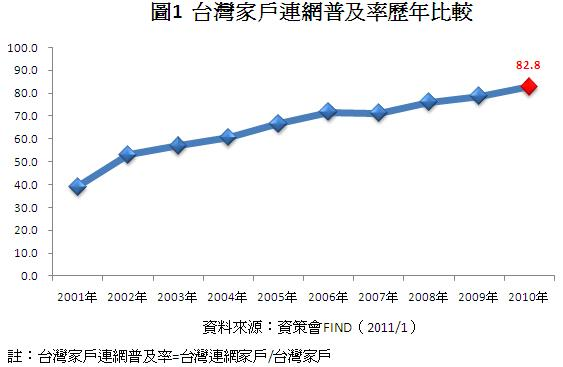
\includegraphics[%
  width=13cm,keepaspectratio]{images/yuwei_2011020901}
\caption{\label{fig:yuwei_2011020901}台灣家戶連網普及率}
%(資料來源:資策會FIND)
\end{figure}

從調查數據~\ref{fig:yuwei_2011022005}所示可以發現兩個趨勢:首先,上網民眾的網路活動更加活躍,在上下載檔案、從事線上影音等活動,都有相當顯著的成長,其次,民眾使用網路交易的比例倍增,顯示民眾對於網路的虛擬購物環境,已有相當程度的信任(資策會)。


\begin{figure}[htbp]
\centering 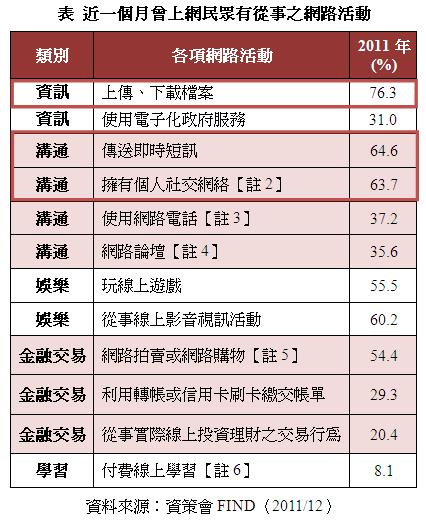
\includegraphics[%
  width=13cm,keepaspectratio]{images/yuwei_2011122005}
\caption{\label{fig:yuwei_2011022005}2011/12月曾上網者之連網使用行為}
%(資料來源:資策會FIND)
\end{figure}

根據以上資料可以了解到近年來網路發展迅速因此消費者習慣也開始改變紛紛改用網路購物因此所謂的『宅經濟』的興起。宅經濟又稱為『閒人經濟』是指不用出門在家就可以從事經濟活動。
根據~\ref{fig:Onlinetrends}臺灣線上購物的市場規模自 2006 年 開始到現今每年 二位數的成長趨勢,2010 年市場規模為 3,583 億元,比 2009 年成長了 15%;預估 2011 年線上購物的市場規模可達到 4,300 億元(資策會 MIC,2010)。他是個成長非常迅速的市場。

\begin{figure}[htbp]
\centering 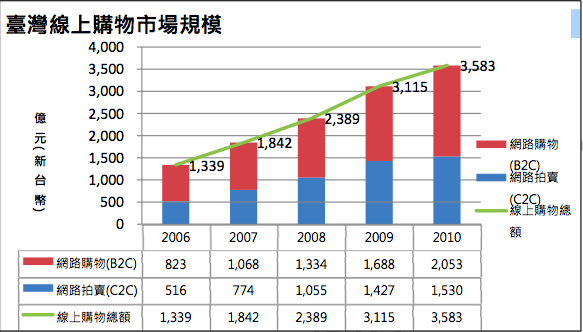
\includegraphics[%
  width=13cm,keepaspectratio]{images/Onlinetrends}
\caption{\label{fig:Onlinetrends}資策會 MIC,2010 台灣線上購物市場規模 3,583 億元,(2012 年 6 月),}
%(資料來源:資策會FIND)
\end{figure}

因此據以上資料來看可以看網路行銷推成出新,在近年來網路社交興起公司紛紛採取社群網站來提升公司的知名度或來作公司產品行銷因此近年產生出新的詞『社群媒體行銷』,觀察網友在最近很火紅的Facebook使用行為上,發現網友使用Facebook的平均使用時間高達439.5分鐘,平均下來,每天約黏在Facebook上面14.65分鐘,已佔了使用社群網站時間的56.6%(資策會FIND)根據互動行銷機構 Rosetta 調查顯示,全球百大零售商已經有 59%在 Facebook 擁有官方粉絲專頁簡稱粉絲團(羅之盈,2010),由此可見,企業也以觀察到Facebook也是一個強大的行銷手法工具之一,透過粉絲專業可以發展出全新的消費者市場,透過Facebook互通性來迅速散播公司相關資訊與雙向溝通可把從粉絲專頁中的人導入公司網路消費者逐群。

但是因為網路通路與實體通路不同的地方是,網路通路所販售的所有商品並不像實體通路有專人解說介紹商品,網路上的消費者只能透過網頁瀏覽器(Web)來觀看網頁上所想購買的商品並沒辦法隨時有像實體通路有專人銷售員介紹的每項功能或使用方法,企業也無法有效掌握顧客的所有需求與企業消費者對商品的滿意度,所以更難推測出未來顧客的消費者行為。



\section{研究目的}
本研究目的是在瞭解透過網路多媒體行銷後的廠商,在網路品牌聲望與品牌知覺是否會影響消費者行為進行分析與推測,提供企業在網路多媒體行銷方面提供有效的建議可以透過本研究更瞭解網路消費者所需求與提升未來企業經營網路虛擬通路之參考


\section{研究流程}

 本研究之流程如圖所示,步驟如下:

1.確定研究動機與範圍

         本研究目的主要目的要探討品牌知覺、品牌聲望、與網路消費者購買行為之關係,研究範圍界定於台灣地區的網路消費者在網路購物中於鈦鍺時尚精品之交易行為。

2-1.文獻收集與研讀

        瞭解本研究的界定主範圍後,開始收集品牌知覺、品牌聲望、網路消費者購買行為、鈦鍺時尚精品等相關文獻,作為研究的基本理論。

2-2. 進行實地訪談

        為了瞭解本研究的鈦鍺時尚精品,相關公司所遇到的問題與消費者行為,前往La Jolla 樂活雅 鈦鍺精品公司實地訪談。

3-1.發展問卷架構

       本研究經過文獻資料與整理及研究探討之後,根據文獻資料與本研究的方向,建立其問卷研發與架構及研究變數,再來針對各個本研究的變數建立研究假設與操作性定義。

3-2.客群分析與訪查

      經過實地親自探訪收集La Jolla 樂活雅 鈦鍺精品公司,所得知的相關客群資料後開始客群分析與訪查本研究相關資料。

4.問卷制作與發放

      本研究方式是採用發放問卷的研究方式,對研究對象進行相關資料的調查;根據研究資料與本研究主題下去研究設計製做問卷,依據本研究該需要的變數去設計選題,即可以開始發放本研究正式的調查問卷,其問卷為網際網路發放方式為收集為主,研究流程如圖~\ref{fig:NPC12}所示。

5.問卷整理與數據分析

      首先針對本研究收回的問卷樣本作敘述性統計分析,了解問卷樣本的基本特性

6.結論與探討

     依據本研究分析後研究出的結果,統整成文後作研究結論與探討,以作為後續與本文相關研究學者與人員參考之文獻

\begin{figure}[htbp]
\centering 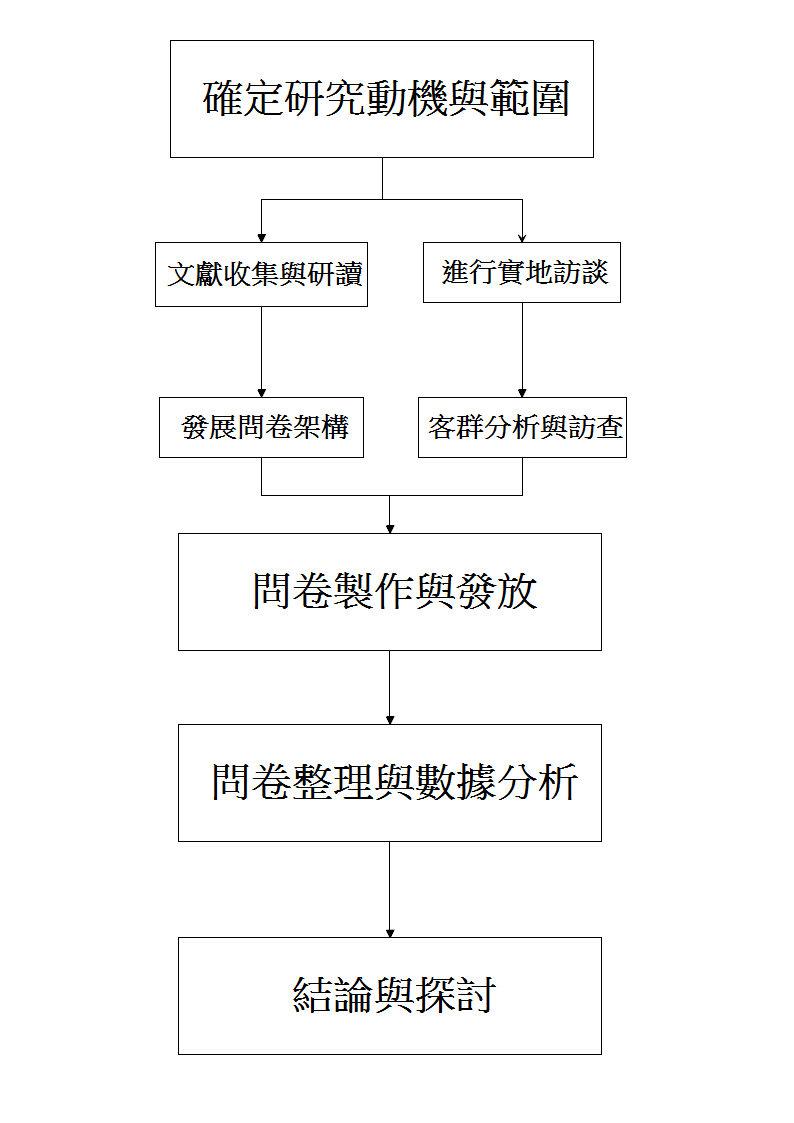
\includegraphics[%
  width=13cm,keepaspectratio]{images/NPC12}
\caption{\label{fig:NPC12}研究流程}
%(資料來源:本研究整理)
\end{figure}



%\section{研究架構}


%\chapter{文獻探討}
%\section{NFC}
%\section{理性行為理論}
%\section{科技接受模式}
%\section{便利性}
%\section{系統品質}
%\section{認知安全性}
%\section{相容性}
%\section{社會影響力}
%
%\chapter{研究設計與方法}
%\section{研究架構}
%\section{研究假說}
%\section{研究構面之操作型定義與衡量問項}
%\section{研究對象}
%\section{資料分析}
%
%\chapter{資料分析與實證研究}
%
%\section{敘述統計分析}
%\section{信度分析}
%\section{建構效度}
%\section{相關分析}
%\section{迴歸分析}
%
%\chapter{研究結論與建議}
%
%\section{研究結論}
%\section{研究貢獻}
%\section{後續研究之建議}
%

\chapter{文獻探討}


\section{品牌聲望}

一、品牌的定義

美國行銷學會(American Medical Association,AMA)
對品牌的定義為:名稱 (Name)詞語(Term) 標記(Sign)象徵(Symbol )設計(design)


\section{品牌知覺}
Aaker (1990) 將消費者對品牌的知覺品質定義為消費者對於某一 項品牌產品整體品質的認知(水)準,或消費者對在(特)定目的下相對於其他品牌, 對某品牌產品或服務全面品質的主觀滿意程度。

kelle(1993)認為品牌認知是指在消費者記憶中較強的品牌聯想與連接。Aacker(1991)認為,

Dawar and Parker(1994) 指出消費者挑選產品以品牌聲望為主要考量
Herbig and Milewica(1996) 正向的品牌聲望有助收益增加。
Kowallczyk and Pawlish(2002)公司聲望是影響消費者購買的因屬之一。
Veloutsou and Moutinho(2009)維持和提升公司聲望比強化消費者滿意度更重要
Priporas and Kamenidou(2011)品牌聲望佈警示品牌保證,也是行銷推廣的利器
\section{品牌行銷}

keller (1998)提出可以從四種角度說明品牌的意義與功能\cite{Aaker}

1.品牌可以用圖案來辨別,可用來與競爭者來區別

2.品牌一致的保證與承諾,是消費者在購買或使用之前的感覺產品的價值與品質

3.品牌是可以自我投射形象,品牌個性的傳達

4.品牌是一組是有關產品的定位,代表一致性品質與功能性的集合,可作為消費者決策購買時的線索

Aaker (1996) 認為品牌權益可分為:(1)品牌知名度 (Brand Awareness)、(2)品牌忠誠度 (Brand loyalty) 、(3)品牌知覺品質 (Brand perceived quality) 、(4)品牌聯想 (Brand Association)、(5)其他品牌專屬資產 (Brand Speciality Asset) 。
    Keller (1998)亦詳細地指出,品牌權益實包含:(1)品牌鮮明度 (Brand Salience):可能會影響消費的判別難易度,(2)品牌績效 (Brand Performance):可以滿足消費者所需功能,(3)品牌形象 (Brand Image):在消費者心中產生對品牌抽象整體概念,(4)品牌判斷 (Brand Judgment) :消費者對於品牌理性層面的判定,(5)品牌情感 (Brand Feeling):消費者對品牌情感的概念與特性,或是社會認可的特徵,(6)品牌共鳴 (Brand Resonance):與消費者品牌關係的最高層次,是由品牌情感到具體行動購買的具體表現,例如主動參與及重複購買的行為忠誠度。

\begin{figure}[htbp]
\centering 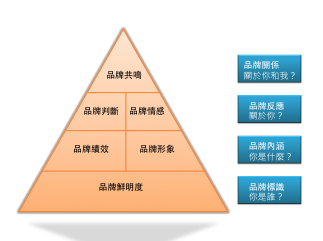
\includegraphics[%
  width=13cm,keepaspectratio]{images/keller2008}
\caption{\label{fig:keller}來自keller2008}
%(資料來源:本研究整理)
\end{figure}


\section{消費者行為}
早期的消費者行為通常都以消費者動機來當研究核心,隨著各位學者長年研究下來提出了許多相關理論的模式,但是現在研究後期主要都已決策的過程為主要核心


%如圖整理~\ref{fig:Consumer1}

%如圖整理~\ref{fig:Consumer2}

\begin{figure}[htbp]
\centering 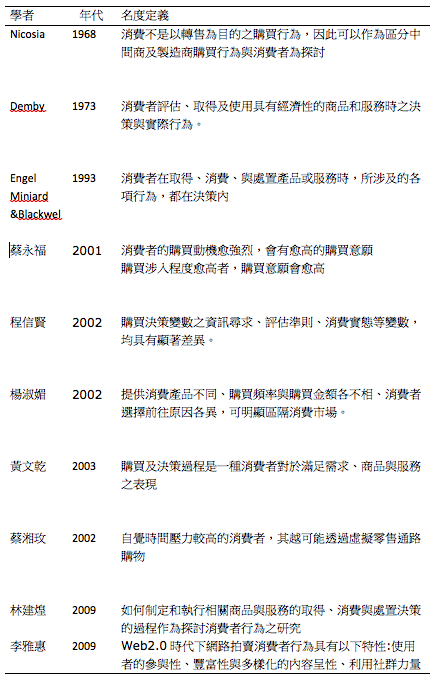
\includegraphics[%
  width=13cm,keepaspectratio]{images/Consumer1}
\caption{\label{fig:Consumer1}本研究整理}
%(資料來源:本研究整理)
\end{figure}

\begin{figure}[htbp]
\centering 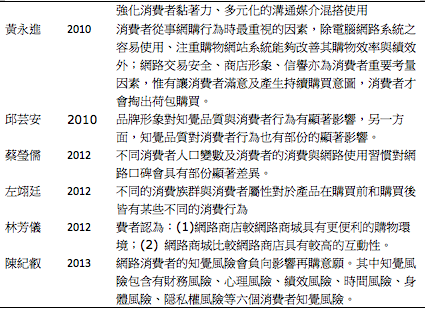
\includegraphics[%
  width=13cm,keepaspectratio]{images/Consumer2}
\caption{\label{fig:Consumer2}本研究整理}
%(資料來源:本研究整理)
\end{figure}



\section{消費者行為理論(Consumer Behavior Theory)}
\subsection{消費者行為定義}
消費者
\begin{figure}[htbp]
\centering 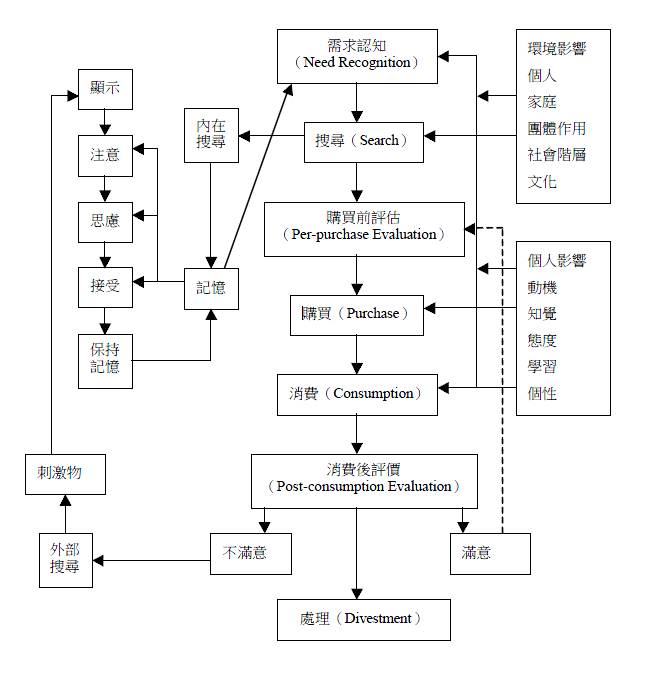
\includegraphics[%
  width=13cm,keepaspectratio]{images/ConsumerBehaviorTheory}
\caption{\label{fig:ConsumerBehaviorTheory}RogerD. Blackwel、PaulW.Miaiard、JamesF.Engel ,CONSUMER  BEHAVIOR,Harcout College Publishers,P38}
%(資料來源:本研究整理)
\end{figure}

\subsection{購買意願之購買決策過程}
Engel, et al (2001) 認為,消費者決策過程的五個重要階段如圖~\ref{fig:Engel}

1.問題認知

購物過程開始時於消費者觀察自身需求與問題來源的認知 ;消費者在問題認知方面會受到外在因素影響(文化,人口統計變數,慘考群體)與個人因刺激,引起消費者產生動機

2.尋求

消費者在確定自己本身所需後,會根據自身問題或是所需來尋求相關資訊,以進行購物決策。一般的消費者收集資訊通常都分為兩種來源,內部搜尋與外部搜尋;消費者,通常會先從自身的記憶中搜尋所需的相關資訊,如過記憶中沒有相關記憶就會改以外部搜尋,獲得協助決策的相關資訊,外部搜尋的資訊如:家人,朋友,廣告,網路等。
           
3.方案評估

搜尋資料完後,就可以對所需要的選著方案做評估與最後的決策。通常消費者都是夠過各項評估的標準與尺度來評定購買的方案。

4.選擇

經過以上敘述方案評估過程後,消費者會以全部方案中選擇最適合的方案,並購買的行動。

5.結果 

當消費者購買產品後,因為本身對產品的期望結果與實際使用的結果,兩種之間的感覺受差異。
一般消費者購買的商品使用後心裡的感受主要有三中結果

符合期望:消費者使用購買的產品後的結果表現符合預期的期望,沒有特別好或壞的感覺

非常滿意:消費者使用購買的產品後的結果表現超過預期的期望,導致心裡的感覺很滿意

不滿意:消費者使用購買的產品後的結果表現低於預期的期望,導致心裡的感覺很不滿意的反應

\begin{figure}[htbp]
\centering 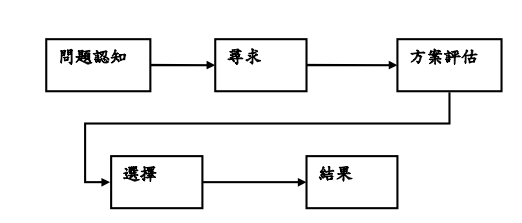
\includegraphics[%
  width=13cm,keepaspectratio]{images/Engel}
\caption{\label{fig:Engel}Engel, et al (2001)}
%(資料來源:本研究整理)
\end{figure}

\subsection{消費者行為理論介紹}

\section{La jolla樂活雅}

公司簡介:

經營據點:台灣:台北市大安區光復南路446號七樓 
               美國:2231 N. 23rd St. Beaumont, TX 77706

 經營理念:富紳國際實業有限公司主要從事首飾及貴金屬零售業;擁有為數不少的客戶群。
最初,是由兩位業餘華裔設計師,自行創作手工珠寶藝品,由於設計風格獨特,大受消費者的歡迎及喜愛,總是供不應求。設計師們有鑑於手工飾品無法大量生產,又觀察到,在未來的飾品趨勢中,鈦飾品將取代金銀等貴重金屬,成為高級珠寶設計重要材質,因此決定發展鈦鍺飾品。

以生產設計鈦鍺精品為主的富紳國際,也接受客戶OEM及ODM訂單。舉凡項鍊、手鍊、戒指、袖扣等商品,並供貨給日本、美國等客戶及珠寶精品業者。
另外,富紳國際亦提供客製化服務,承接結合鈦飾品及頂級鑽石之客製化訂單,為消費者
提供獨一無二的商品訂製服務。

發展至今,富紳國際已擁有自己的設計師及協力生產工廠,從來圖打樣、來樣製作及專業生產一應俱全。專屬設計師群發揮豐富的創造力,賦與每一款設計精品獨創的理念,再結合老師傅精湛的珠寶鑲工技藝,精心打造每一分一毫細微處,提供國內外客戶最與眾不同、匠心獨具的頂級鈦鍺珠寶精品。

 企業文化:La Jolla品牌概念來自於美國加州。 La Jolla,源於西班牙文「珠寶」之意-「聖地牙哥的海洋之珠」,因為是西班牙文,所以唸法獨特,J的發音為H的氣音,唸作[ la-ho-ya](接近中文發音”拉荷亞)。La Jolla是一個位於美國加州San Diego的明媚小鎮。

在「陽光.沙灘.美麗海岸」的見證下,品牌創辦人遇見了”命中注定”的另一半,並於 La Jolla
小鎮買下了別具意義的定情戒,兩人互許真愛,相守一生。這份難能可貴的愛情,讓他們
決心將這份浪漫,轉化為璀燦迷人的健康概念純鈦飾品,將他們勇於追尋真愛的故事,透
過La Jolla精品,不斷的傳遞出去。

La Jolla品牌理念-Pure and  Trendy

Pure 材質純度嚴選 

Trendy 引領現代時尚精品風格 

「 La Jolla期許能結合藝術、自然、愜意美好的一切事物,以獨到細膩的品味設計、純鈦
的材質,帶來對生命最美好的感動。」 有別於一般市售的大眾化純鈦飾品, La Jolla
品牌創辦人堅持自我品味,精心打造一個具有現代時尚個性的純鈦精品。旗下專業設計師
更以獨創的設計理念,賦與每款飾品生命力,並結合老師傅細緻的鑲工手藝,極致講究每
一分每一毫細微的作工,呈現出純鈦精品的高雅質感及活力,演繹品味獨具的 La Jolla
純鈦精品新魅力。
                                                                                      
                             by品牌創辦人CORA LIU
(資料來源:La Jolla 樂活雅鈦鍺精品)
 
品牌故事

有別於一般市售的大眾化鈦鍺飾品,La Jolla品牌創辦人CORA LIU堅持自我品味,精心打造一個具有現代時尚個性的鈦鍺精品。旗下專業設計師更以獨創的設計理念,賦與每款飾品生命力,並結合老師傅細緻的鑲工手藝,極致講究每一分每一毫細微的作工,呈現出鈦鍺飾品的高雅質感及活力,演繹品味獨具的La Jolla鈦鍺精品新魅力。

\begin{figure}[htbp]
\centering 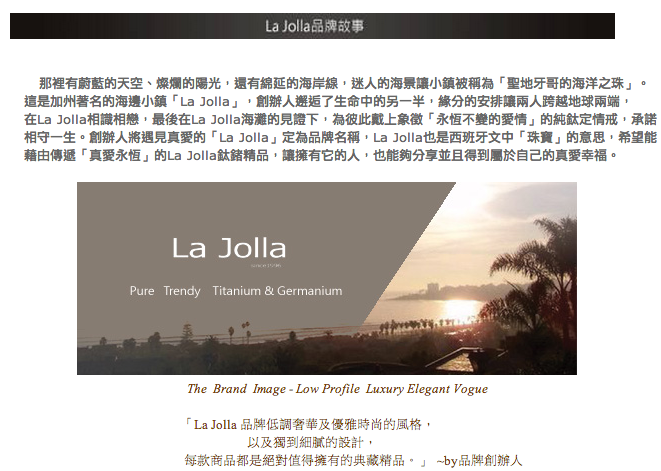
\includegraphics[%
  width=13cm,keepaspectratio]{images/LaJolla}
\caption{\label{fig:LaJolla}LaJolla樂活雅鈦鍺精品}
%(資料來源:本研究整理)
\end{figure}



\chapter{研究假設與架構}
\section{概念架構}
本研究根據文獻探討的回顧與整理,建立研究之架構如圖:\ref{fig:ARC}所以本研究探討品牌知覺與品牌聲望與網路消費者決策和消費者滿意度之間的關係,暸解品牌聲望與品牌知覺對網路消費者決策與網路消費者滿意度之研究,並建立本研究架構。


\begin{figure}[!t]
\centering
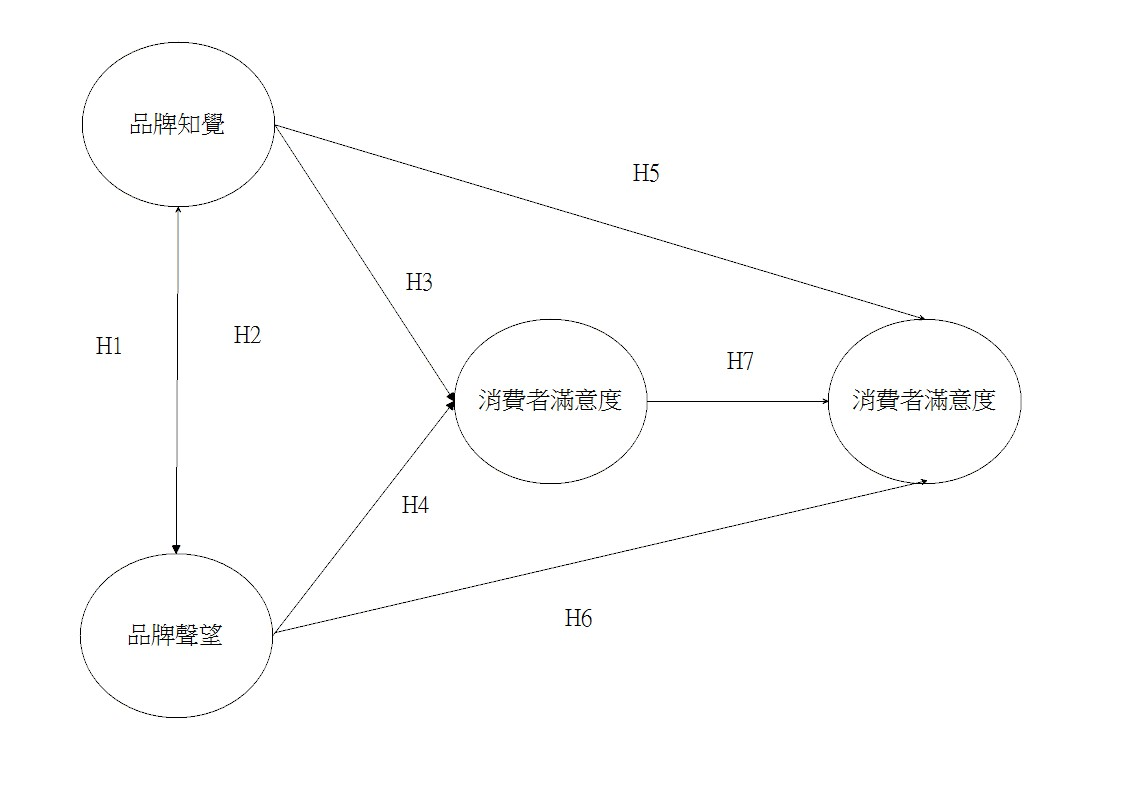
\includegraphics[width=14cm]{images/論文架構.jpg}
\caption{研究架構}
\label{fig:ARC}
\end{figure}

\section{研究假設}
根據上述的的目的,本研究嘗試提出以 下假設:
\begin{enumerate}
\item 根據Aaker (1991) 將消費者對品牌的知覺品質定義為消費者對於某一 項品牌產品整體品質的認為水準,或消費者對在特定目的下相對於其他品牌, 對某品牌產品或服務全面品質的主觀滿意程度,基於以上的推論,本研究提出以下的研究假設 :

H1品牌知覺會正向影響品牌聲望有顯著的關係

H2品牌聲望會正向影響品牌知覺有顯著的關係

\item 根據 Rao and Ruekert (1994) 品牌對於消費者而言是屬於產品的一部分,可視為傳遞產品品質訊息的媒介,而且往往是消費者購買決策的重要考量因素之一,基於以上的推論,本研究提出以下的研究假設 :

H3品牌知覺會正向影響消費者決策有顯著的關係

H4品牌聲望會正向影響消費者決策有顯著的關係

\item 根據藍悅真(2012)指出品牌會影響消費者滿意度,Oliver (1980) 指出消費者如之前購買經驗是否感到滿意,而決定是否再次購買;基於以上的推論,本研究提出以下的研究假設 :

H5品牌知覺會正向影響消費者滿意度有顯著的關係

H6品牌聲望會正向影響消費者滿意度有顯著的關係

H7消費者決策會正向影響消費者滿意度有顯著的關係

\end{enumerate}

\section{研究對象與抽樣方法}
本研究目的主要探討品牌知覺,品牌聲望對消費者決策與消費者滿意度之關係,並提出對公司意見與建議,以網路使用者為受訪為樣本,問卷蒐集方式採用Google Docs「網路問卷調查表」以網路散播方式發放。

本研究共有五大部份,第一部分蒐集樣本的性別、年齡等人口統計變數資料,後前四部分均以李克特(Lilert)五點尺度量表來 衡量(1=非常不同意,2=不同意,3=不同意也非不同意,4=同意,5=非常同意)。
第二部分衡量消費者決策共10題,第三部分衡量品牌知覺共有8題,第四部分衡量品牌聲望共有10題,第五部分衡量消費者滿意度共有10題

\section{變數的定義與衡量}
\begin{enumerate}
\item  網路消費者決策共有10個題目在網路上選購精品、珠寶商品時會參考的因素:價錢、品牌形象、製造材料與特性、其他顧客反應度、商品認證保證、售後服務、交貨服務、整體商品的價值、品牌知名度、設計感
\item 品牌知覺共有8個題目知覺對鈦鍺的所產生出來的狀況:商品的品質良好、鈦鍺品牌形象、製作材料(與特性)、商品外觀設計很滿意、商品的廣告或名稱很滿意、整體商品的價值、品牌知名度
\item 品牌聲望共有10個題目得到相關資訊是否有幫助您了解LaJolla鈦鍺精品:價錢、品牌形象、製作材料(與特性)、其他顧客反應、商品認證保證、售後服務、交貨服務、整體商品的價值、品牌知名度、設計感
\item 消費者滿意度共有10題目購買相關LaJolla鈦鍺精品的滿意度:價錢、品牌形象、製作材料(與特性)、其他顧客反應、商品認證保證、售後服務、交貨服務、整體商品的價值、品牌知名度、設計感
\end{enumerate}

\section{資料分析方法}
本研究利用統計分析套件軟體 SPSS 20進行相關分析,使用的分析如下
\begin{enumerate}
\item 描述性統計 :分析樣本結構中性別,年紀教育,程度工作性質的百分比
\item 信度分析:以Cronbach's 值來鑑定各量表的內部一致性
\item 因素分析:主要目的將原有很多變數(維度)之資料,縮減成較少的維度數,但有保持原本所提供的資料
\item 簡單迴歸:分析進行假設的驗證
\end{enumerate}

本研究探討品牌知覺、品牌聲望、消費者滿意度之間的關係。本研究已發放問卷的方式取的資料,問卷填寫主要以網路發放題目主要
品牌知覺、品牌聲望、消費者滿意度以簡單迴歸分析來驗證假設是否成立

\chapter{研究結果展示}
\section{敘述統計}
本研究採用網路與百貨公司附近發放方式,針對可能聽過鈦鍺精品的人進行問卷調查供調查603份剔除重複填寫與漏填,有效問卷599份 
本研究的樣本資料分析結果顯示 
\begin{enumerate}
\item 男性佔 50.4 % 女性 49.6% 如表 \ref{tab:PL1} 所示 
\item 年齡分為18歲以下 9.7% 、19 ~25歲 72.0% 、26~35歲 9.8%、36~40歲2.7% 、40歲以上5.8%本問卷族群與年輕族群居多。如表  \ref{tab:PL2} 所示
\item 教育方面 高中以下4.1%、高中(職)19.2%、專科5.3%、大學63.7%、碩士5.3%、博士1.7% 教育程度以大學64.7%為最多 。如表 \ref{tab:PL3} 所示
\item 工作性質 學生52.8%、服務業29.5%、製造業3.5%、軍公教4.3%、自由業8.5%、管家1.3%由職業可看以學生64.7%為最高。如表 \ref{tab:PL4} 所示
\end{enumerate}

\begin{table}[htb]
\caption{敘述統計(性別)}
\label{tab:PL1}
\renewcommand{\arraystretch}{1.2} % 將表格行間距加大為原來的 1.2 倍
\arrayrulewidth=1pt               % 調整線條粗細為 1pt
\tabcolsep=60pt                   % 調整欄間距為 24pt
%\begin{document}
\begin{tabular}[t]{lll}  % 第一欄位使用 sans serif 字族
\hline
 性別&次數 & 百分比 \\
\hline
男生        & 302 & 50.4 \\
女生        & 297  & 49.6 \\
總和        & 599  & 100 \\
\hline
\centering
\label{fig:PL4}
\end{tabular}
\end{table}

\begin{table}[htb]
\caption{敘述統計(年齡)}
\label{tab:PL2}
\renewcommand{\arraystretch}{1.2} % 將表格行間距加大為原來的 1.2 倍
\arrayrulewidth=1pt               % 調整線條粗細為 1pt
\tabcolsep=60pt                   % 調整欄間距為 24pt
%\begin{document}
\begin{tabular}[t]{lll}  % 第一欄位使用 sans serif 字族
\hline
 年齡& 次數 & 百分比 \\
\hline
18歲以下        & 58  & 9.7 \\
19~25歲        & 431  & 72.0 \\
26~35歲        & 59  & 9.8 \\
36~40歲        & 16  &2.7\\
40歲以上        & 35  & 5.8 \\
總和               & 599  & 100 \\
\hline
\end{tabular}
\end{table}

\begin{table}[htb]
\caption{敘述統計(學歷)}
\label{tab:PL3}
\renewcommand{\arraystretch}{1.2} % 將表格行間距加大為原來的 1.2 倍
\arrayrulewidth=1pt               % 調整線條粗細為 1pt
\tabcolsep=60pt                   % 調整欄間距為 24pt
%\begin{document}
\begin{tabular}[t]{lll}  % 第一欄位使用 sans serif 字族
\hline
 學歷& 次數 & 百分比 \\
\hline
高職以下       & 25  & 4.2 \\
高中(職)        & 116  &19.4\\
專科        & 32  & 5.3 \\
大學        & 384 &64.1\\
碩士        & 32  & 5.3 \\
博士           & 10  & 1.7 \\
總和           & 599  & 100 \\
\hline
\end{tabular}
\end{table}

\begin{table}[htb]
\caption{敘述統計(工作性質)}
\label{tab:PL4}
\renewcommand{\arraystretch}{1.2} % 將表格行間距加大為原來的 1.2 倍
\arrayrulewidth=1pt               % 調整線條粗細為 1pt
\tabcolsep=60pt                   % 調整欄間距為 24pt
\begin{tabular}[t]{lll}  % 第一欄位使用 sans serif 字族
\hline
 工作性質& 次數 & 百分比 \\
\hline
學生           & 316  & 52.8 \\
服務業        & 177  & 29.5 \\
製造業        & 21  & 3.5 \\
軍公教        & 26  &4.3\\
自由業        & 51  & 8.5 \\
家管           & 8  & 1.3 \\
總和               & 599  & 100 \\
\hline
\end{tabular}
\end{table}

\section{信度分析}
首先對樣本收集已說明,其次對本研究的變數衡量做信度分析最後驗證假設
信度分析:已進行實證分析針對問卷問項進行信度分析用來得知問卷設計所測得的結果是否有信度與穩定性本研究採用目前已研究最常使用的 信賴度數做信度量測指標 Nunnally(1978)認為信度0.7以上表示高信度 可接受值大於0.7

本研究共有 3個變數,信度分析結果顯示
\begin{enumerate}
\item 消費者決策Cronbach's Alpha 值 0.946  如表 \ref{tab:e1}  所示
\item 品牌知覺Cronbach's Alpha 值 0.936  如表 \ref{tab:e2}  所示
\item 品牌聲望Cronbach's Alpha 值  0.958 如表 \ref{tab:e3}  所示
\item 消費者滿意度Cronbach's Alpha 值 0.969 如表 \ref{tab:e4}  所示
\end{enumerate}
以上信度 Alpha 值 大於 0.7以上顯示本研究的變數具有不錯的可信度。

\begin{table}[htb]
\caption{信度 (消費者決策)}
\label{tab:e1}
\renewcommand{\arraystretch}{1.2} % 將表格行間距加大為原來的 1.2 倍
\arrayrulewidth=1pt               % 調整線條粗細為 1pt
\tabcolsep=18pt                   % 調整欄間距為 24pt
\begin{tabular}[t]{lllll}  % 第一欄位使用 sans serif 字族
\hline
  & 代號& 平均數 & 標準差&  Alpha 值  \\
\hline
消費者決策&決策1&3.9873&0.82930&0.945735\\
               &決策2&3.9429	&0.82742&\\	
               &決策3&3.9460&0.81796&\\
               &決策4&3.9143&0.85713&\\
               &決策5&4.0540&0.82955&\\
               &決策6&4.0476&0.84515&\\
               &決策7&3.9905&0.83508&\\
               &決策8&4.0413&0.83792&\\
               &決策9&3.8381&0.86094&\\
               &決策10&3.9905&0.86136&\\
\hline
\end{tabular}
\end{table}

\begin{table}[htb]
\caption{信度 (品牌知覺)}
\label{tab:e2}
\renewcommand{\arraystretch}{1.2} % 將表格行間距加大為原來的 1.2 倍
\arrayrulewidth=1pt               % 調整線條粗細為 1pt
\tabcolsep=18pt                   % 調整欄間距為 24pt
\begin{tabular}[t]{lllll}  % 第一欄位使用 sans serif 字族
\hline
 & 代號& 平均數 & 標準差&  Alpha 值  \\
\hline
品牌知覺 & 知覺1  & 3.7753   & 0.7479  &0.936242 \\
              & 知覺2  & 3.7483  &0.79497  &  \\
             & 知覺3  & 3.8345    & 0.80373  &  \\
             & 知覺4 & 3.7500   &0.75513  &\\
             & 知覺5   & 3.7534  & 0.77393 &  \\
             & 知覺6  & 3.7534    &  0.77393 & \\
             & 知覺7  & 3.6909     & 0.80231  &  \\
\hline
\end{tabular}
\end{table}


\begin{table}[htb]
\caption{信度 (品牌聲望)}
\label{tab:e3}
\renewcommand{\arraystretch}{1.2} % 將表格行間距加大為原來的 1.2 倍
\arrayrulewidth=1pt               % 調整線條粗細為 1pt
\tabcolsep=18pt                   % 調整欄間距為 24pt
\begin{tabular}[t]{lllll}  % 第一欄位使用 sans serif 字族
\hline
 & 代號& 平均數 & 標準差&  Alpha 值  \\
\hline
品牌知覺 & 聲望1  & 3.6835 &0.82500 &0.958532\\
              & 聲望2  & 3.7089 &0.83439 &  \\
             & 聲望3  &3.6962 &0.85266  &  \\
             & 聲望4  &3.5949&0.75987\\
             & 聲望5  & 3.7468 &0.83924 &  \\
             & 聲望6  & 3.6456&0.78508& \\
             & 聲望7  & 3.6709&0.77900  &  \\
             & 聲望8  & 3.7215&0.84636&  \\
             & 聲望9  &3.6456&0.81709&  \\
             & 聲望10  & 3.7848&0.82696 &  \\
\hline
\end{tabular}
\end{table}

\begin{table}[htb]
\caption{信度 (消費者滿意度)}
\label{tab:e4}
\renewcommand{\arraystretch}{1.2} % 將表格行間距加大為原來的 1.2 倍
\arrayrulewidth=1pt               % 調整線條粗細為 1pt
\tabcolsep=18pt                   % 調整欄間距為 24pt
\begin{tabular}[t]{lllll}  % 第一欄位使用 sans serif 字族
\hline
 & 代號& 平均數 & 標準差&  Alpha 值  \\
\hline
品牌知覺 & 滿意度1&3.233&0.97143&0.969024\\
              & 滿意度2&3.4667&1.10589&  \\
             & 滿意度3&3.5000&1.00858&  \\
             & 滿意度4&3.5667&1.13512&\\
             & 滿意度5&3.7000&1.08755&  \\
             & 滿意度6&3.5667&1.16511&\\
             & 滿意度7&3.4667&1.00801&  \\
             & 滿意度8&3.6333&0.99943&  \\
             & 滿意度9&3.4333&1.04000&\\
             & 滿意度10&3.5667&1.07265&\\
\hline
\end{tabular}
\end{table}

\section{因素分析}
為了探討受訪者對主要考量因素,因此提出10提消費者行為、8題品牌知覺、10題品牌知覺、10題消費者滿意度等變數以量表收集受訪者對每一變數之重視度(非常不同意=1、非常同意=5)。將所獲得之資料,經過KMO取樣適當性及巴氏球形檢定,KMO值越高表示進行因素分析的效果越好,其值在0.9以上表示效果極佳,0.8以上表示是有價值的,0.7以上是中度的,0.6以上是不好也不壞,0.5以上是不太好,若值在0.5以下,就表示其效果是無法接受的
\begin{enumerate}
\item 消費者決策
KMO=0.948 大於0.9表示分析效果極佳 Bartlett 的球形檢值 2427.156 顯著性.000<α = 0.01 顯示資料非常適合因素分析  本部分特性值大於1之標準將10個變數濃縮為1個因變數(主成分)全部變異可解釋為67.400%,詳細的數據如表  \ref{tab:p4} 所示。
\item 品牌知覺
KMO=0.926 大於0.9表示分析效果極佳 Bartlett 的球形檢值 3210.519 顯著性.000<α = 0.01 顯示資料非常適合因素分析  本部分特性值大於1之標準將7個變數濃縮為1個因變數(主成分)全部變異可解釋為72.457%,詳細的數據如表  \ref{tab:p4} 所示。
\item 品牌聲望
KMO=0.899 大於0.8表示分析有價值 Bartlett 的球形檢值 800.032 顯著性.000<α= 0.01 顯示資料有價值因素分析  本部分特性值大於1之標準將10個變數濃縮為1個因變數(主成分)全部變異可解釋為73.020% 如圖 \ref{tab:p4}  所示。
\item 消費者滿意度
KMO=0.788 大於0.7表示分析中等 Bartlett 的球形檢值 420.646 顯著性.000<α=0.01 顯示資料中度合因素分析  本部分特性值大於1之標準將10個變數濃縮為1個因變數(主成分)全部變異可解釋為78.632% 如圖 \ref{tab:p4} 所示
\end{enumerate}

\begin{table}[htb]
\caption{因數分析}
\label{tab:p4}
\renewcommand{\arraystretch}{1.2} % 將表格行間距加大為原來的 1.2 倍
\arrayrulewidth=1pt               % 調整線條粗細為 1pt
\tabcolsep=16pt                   % 調整欄間距為 24pt
\begin{tabular}[t]{lllll}  % 第一欄位使用 sans serif 字族
\hline
 項目& KMO值 & KMO值接受度& 巴氏球型檢定&顯著性 \\
\hline
消費者決策&0.948&效果極佳&2427.156&0.000\\
 品牌知覺&0.926&效果極佳&3210.519&0.000\\
 品牌聲望&0.899&有價值&800.032&0.000 \\
消費者滿意度&0.788&中度&420.646&0.000\\
\hline
\end{tabular}
\end{table}

%\begin{figure}[!t]
%\centering
%\includegraphics[width=8cm]{images/kom.PNG}
%\caption{因素分析}
%\label{fig:p4}
%\end{figure}
\section{假設之驗證}
本研究共有6個假設待驗證,均採用簡單迴歸分析,結果整理於表 \ref{tab:HRR} 所示以下對每個假設驗證結果加以說明
\begin{enumerate}
\item 假設1:品牌知覺會正向影響品牌聲望有顯著的關係。
依簡單迴歸分析得值為:依變數[品牌知覺]R:0.480 R平方:0.231 如表\ref{tab:HR1}  所示。
的迴歸值(B之估計值)為0.468其t值4.678 顯著性值為=0.000<α=0.05,故棄卻其為0之虛無假設,回歸方程式之自變數的係數不為0,自變數與因變數間存在直線關係,因此可看出品牌聲望會正向影響品牌知覺有顯著的關係之假設=成立。 如表\ref{tab:H1}  所示。
\item 假設2:品牌聲望會正向影響品牌知覺有顯著的關係。
依簡單迴歸分析得值為:依變數[品牌聲望]R:0.480 R平方:0.231 如表\ref{tab:HR2}  所示。
迴歸值(B之估計值)為0.492其t值4.678顯著性值為=0.000<α=0.05,故棄卻其為0之虛無假設,回歸方程式之自變數的係數不為0,自變數與因變數間存在直線關係,因此可看出品牌知覺會正向影響品牌聲望有顯著的關係之假設=成立。如表\ref{tab:H2}  所示。
\item 假設3:品牌知覺會正向影響消費者決策有顯著的關係。
以簡單迴歸分析得值為:自變數[消費者決策]R:709 R平方:0.502 如表\ref{tab:HR3}  所示。
迴歸值(B之估計值)為0.665其t值17.572 顯著性值為=0.000<α=0.05,故棄卻其為0之虛無假設,回歸方程式之自變數的係數不為0,自變數與因變數間存在直線關係,因此可看出品牌知覺會正向影響消費者決策有顯著的關係之假設=成立。 如表 \ref{tab:H3}  所示。
\item 假設4:品牌聲望會正向影響消費者決策有顯著的關係。
以簡單迴歸分析得值為:自變數[品牌知覺]R:0.489 R平方:0.239 如表\ref{tab:HR4}  所示。
迴歸值(B之估計值)為0.501其t值4.619 顯著性值為=0.000<α=0.05,故棄卻其為0之虛無假設,回歸方程式之自變數的係數不為0,自變數與因變數間存在直線關係,因此可看出品牌聲望會正向影響消費者決策有顯著的關係之假設=成立。 如表 \ref{tab:H4}  所示。
\item 假設5:品牌知覺會正向影響消費者滿意度有顯著的關係。。
以簡單迴歸分析得值為:自變數[品牌聲望]R:0.495 R平方:0.214 如表\ref{tab:HR5}  所示
迴歸值(B之估計值)為0.422其t值2.846 顯著性值為=0.009<α=0.05,故棄卻其為0之虛無假設,回歸方程式之自變數的係數不為0,自變數與因變數間存在直線關係,因此可看出品牌知覺會正向影響消費者滿意度有顯著的關係之假設=成立。 如表\ref{tab:H5}  所示。
\item 假設6:品牌聲望會正向影響與消費者滿意度有顯著的關係。
以簡單迴歸分析得值為:自變數[消費者行為]R:0.898 R平方:0.798 如表\ref{tab:HR6}  所示。
迴歸值為(B之估計值)為0.712其t值10.390 顯著性值為=0.000<α=0.05,故棄卻其為0之虛無假設,回歸方程式之自變數的係數不為0,自變數與因變數間存在直線關係,因此可看出消費者滿意度與消費者滿意度有顯著的關係之假設=。 如表 \ref{tab:H6}  所示。
\item 假設7:消費者決策會正向影響與消費者滿意度有顯著的關係。
以簡單迴歸分析得值為:自變數[消費者行為]R:0.529 R:0.252如表\ref{tab:HR7}  所示。
迴歸值迴歸值為0.423 其t值3.176 顯著性值為=0.004<α=0.05,故棄卻其為0之虛無假設,回歸方程式之自變數的係數不為0,自變數與因變數間存在直線關係,因此可看出消費者滿意度與消費者滿意度有顯著的關係之假設=。 如表 \ref{tab:H7}  所示。

\end{enumerate}


\begin{table}[htb]
\caption{假設}
\label{tab:HRR}
\centering
\renewcommand{\arraystretch}{1.2} % 將表格行間距加大為原來的 1.2 倍
%\arrayrulewidth=1pt               % 調整線條粗細為 1pt
%\tabcolsep=10pt                   % 調整欄間距為 24pt
\begin{tabular}[t]{lclclclclclclclcl}  % 第一欄位使用 sans serif 字族
\hline
 假設&模型路徑&R&R平方&B之估計值& P值& t& 結果 \\
\hline
H1&品牌知覺→品牌聲望&0.480&0.231&0.468&0.000&4.678&成立\\
H2&品牌聲望→品牌知覺&0.480&0.231&0.492&0.000&4.678&成立\\
H3&品牌知覺→消費者決策&0.709&0.502&0.665&0.000&17.572&成立\\
H4&品牌聲望→消費者決策&0.489&0.239&0.501&0.000&4.619&成立\\
H5&品牌知覺→消費者滿意度&0.495&0.245&0.422&0.009&2.846&成立\\
H6&品牌聲望→消費者滿意度&0.898&0.806&0.712&0.000&10.390&成立\\
H7&消費者決策→消費者滿意度&0.529&0.280&0.423&0.004&3.176&成立\\
\hline
\end{tabular}
\end{table}

\begin{table}[htb]
\caption{簡單回歸R(A.預測變數:知覺B.依變數:聲望)}
\label{tab:HR1}
\centering
\renewcommand{\arraystretch}{1.2} % 將表格行間距加大為原來的 1.2 倍
\arrayrulewidth=1pt               % 調整線條粗細為 1pt
\tabcolsep=10pt                   % 調整欄間距為 24pt
\begin{tabular}[t]{lclclclclclcl}  % 第一欄位使用 sans serif 字族
\hline
 模型&R&R平方&調整後R平方&估計的標準誤差&顯著性\\
\hline
&0.480&0.231&0.220&0.88418990&0.000\\
\hline
\end{tabular}
\end{table}


\begin{table}[htb]
\caption{簡單回歸(依變數:聲望構面)}
\label{tab:H1}
\centering
\renewcommand{\arraystretch}{1.2} % 將表格行間距加大為原來的 1.2 倍
\arrayrulewidth=1pt               % 調整線條粗細為 1pt
\tabcolsep=10pt                   % 調整欄間距為 24pt
\begin{tabular}[t]{lclclclclclcl}  % 第一欄位使用 sans serif 字族
\hline
 模型&B估計值&標準誤差&Beta分配&t&顯著性\\
\hline
(常數)&-0.119&0.105&&-1.133&0.261\\
知覺的構面&0.468&0.100&0.480&4.678&0.000\\
\hline
\end{tabular}
\end{table}


\begin{table}[htb]
\caption{簡單回歸R(A.預測變數:聲望B.依變數:知覺)}
\label{tab:HR2}
\centering
\renewcommand{\arraystretch}{1.2} % 將表格行間距加大為原來的 1.2 倍
\arrayrulewidth=1pt               % 調整線條粗細為 1pt
\tabcolsep=10pt                   % 調整欄間距為 24pt
\begin{tabular}[t]{lclclclclclcl}  % 第一欄位使用 sans serif 字族
\hline
 模型&R&R平方&調整後R平方&估計的標準誤差&顯著性\\
\hline
&0.480&0.231&0.220&0.90642769&0.000\\
\hline
\end{tabular}
\end{table}

\begin{table}[htb]
\caption{簡單回歸(依變數:知覺構面)}
\label{tab:H2}
\centering
\renewcommand{\arraystretch}{1.2} % 將表格行間距加大為原來的 1.2 倍
\arrayrulewidth=1pt               % 調整線條粗細為 1pt
\tabcolsep=10pt                   % 調整欄間距為 24pt
\begin{tabular}[t]{lclclclclclcl}  % 第一欄位使用 sans serif 字族
\hline
 模型&B估計值&標準誤差&Beta分配&t&顯著性\\
\hline
(常數)&0.249&0.105&&2.375&0.020\\
聲望的構面&0.492&0.105&0.480&4.678&0.000\\
\hline
\end{tabular}
\end{table}


\begin{table}[htb]
\caption{簡單回歸R(A.預測變數:知覺B.依變數:決策)}
\label{tab:HR3}
\centering
\renewcommand{\arraystretch}{1.2} % 將表格行間距加大為原來的 1.2 倍
\arrayrulewidth=1pt               % 調整線條粗細為 1pt
\tabcolsep=10pt                   % 調整欄間距為 24pt
\begin{tabular}[t]{lclclclclclcl}  % 第一欄位使用 sans serif 字族
\hline
 模型&R&R平方&調整後R平方&估計的標準誤差&顯著性\\
\hline
&0.709&0.502&0.501&0.68984431&0.000\\
\hline
\end{tabular}
\end{table}


\begin{table}[htb]
\caption{簡單回歸(依變數:決策的構面)}
\label{tab:H3}
\centering
\renewcommand{\arraystretch}{1.2} % 將表格行間距加大為原來的 1.2 倍
\arrayrulewidth=1pt               % 調整線條粗細為 1pt
\tabcolsep=10pt                   % 調整欄間距為 24pt
\begin{tabular}[t]{lclclclclclcl}  % 第一欄位使用 sans serif 字族
\hline
 模型&B估計值&標準誤差&Beta分配&t&顯著性\\
\hline
(常數)&-.077&0.040& &-1.949&0.052\\
知覺的構面&0.665&0.038&0.709&17.572&0.000\\
\hline
\end{tabular}
\end{table}

\begin{table}[htb]
\caption{簡單回歸R(A.預測變數:聲望B.依變數:決策)}
\label{tab:HR4}
\centering
\renewcommand{\arraystretch}{1.2} % 將表格行間距加大為原來的 1.2 倍
\arrayrulewidth=1pt               % 調整線條粗細為 1pt
\tabcolsep=10pt                   % 調整欄間距為 24pt
\begin{tabular}[t]{lclclclclclcl}  % 第一欄位使用 sans serif 字族
\hline
 模型&R&R平方&調整後R平方&估計的標準誤差&顯著性\\
\hline
&0.489&0.239&0.228&0.9254205&0.000\\
\hline
\end{tabular}
\end{table}


\begin{table}[htb]
\caption{簡單回歸(依變數:決策的構面)}
\label{tab:H4}
\centering
\renewcommand{\arraystretch}{1.2} % 將表格行間距加大為原來的 1.2 倍
\arrayrulewidth=1pt               % 調整線條粗細為 1pt
\tabcolsep=10pt                   % 調整欄間距為 24pt
\begin{tabular}[t]{lclclclclclcl}  % 第一欄位使用 sans serif 字族
\hline
 模型&B估計值&標準誤差&Beta分配&t&顯著性\\
\hline
(常數)&-.108&0.111& &-.975&0.333\\
聲望的構面&0.501&0.108&0.489&4.619&0.000\\
\hline
\end{tabular}
\end{table}


\begin{table}[htb]
\caption{簡單回歸R(A.預測變數:知覺B.依變數:滿意度)}
\label{tab:HR5}
\centering
\renewcommand{\arraystretch}{1.2} % 將表格行間距加大為原來的 1.2 倍
\arrayrulewidth=1pt               % 調整線條粗細為 1pt
\tabcolsep=10pt                   % 調整欄間距為 24pt
\begin{tabular}[t]{lclclclclclcl}  % 第一欄位使用 sans serif 字族
\hline
 模型&R&R平方&調整後R平方&估計的標準誤差&顯著性\\
\hline
&0.495&0.245&0.214&0.90732819&0.009\\
\hline
\end{tabular}
\end{table}

\begin{table}[htb]
\caption{簡單回歸(依變數:滿意度構面)}
\label{tab:H5}
\centering
\renewcommand{\arraystretch}{1.2} % 將表格行間距加大為原來的 1.2 倍
\arrayrulewidth=1pt               % 調整線條粗細為 1pt
\tabcolsep=10pt                   % 調整欄間距為 24pt
\begin{tabular}[t]{lclclclclclc|}  % 第一欄位使用 sans serif 字族
\hline
 模型&B估計值&標準誤差&Beta分配&t&顯著性\\
\hline
(常數)&-.044&0.175&&-254&0.802\\
知覺的構面&0.422&0.148&0.495&2.846&0.009\\
\hline
\end{tabular}
\end{table}

\begin{table}[htb]
\caption{簡單回歸R(A.預測變數:聲望B.依變數:滿意度)}
\label{tab:HR6}
\centering
\renewcommand{\arraystretch}{1.2} % 將表格行間距加大為原來的 1.2 倍
\arrayrulewidth=1pt               % 調整線條粗細為 1pt
\tabcolsep=10pt                   % 調整欄間距為 24pt
\begin{tabular}[t]{lclclclclclc|}  % 第一欄位使用 sans serif 字族
\hline
 模型&R&R平方&調整後R平方&估計的標準誤差&顯著性\\
\hline
&0.898&0.806&0.798&0.46030781&0.000\\
\hline
\end{tabular}
\end{table}

\begin{table}[htb]
\caption{簡單回歸(依變數:滿意度構面)}
\label{tab:H6}
\centering
\renewcommand{\arraystretch}{1.2} % 將表格行間距加大為原來的 1.2 倍
\arrayrulewidth=1pt               % 調整線條粗細為 1pt
\tabcolsep=10pt                   % 調整欄間距為 24pt
\begin{tabular}[t]{lclclclclclc|}  % 第一欄位使用 sans serif 字族
\hline
 模型&B估計值&標準誤差&Beta分配&t&顯著性\\
\hline
常數&0.171&0.089&&1.912&0.067 \\
聲望的構面 & 0.712 & 0.069 & 0.898 & 10.390 & 0.000 \\
\hline
\end{tabular}
\end{table}


\begin{table}[htb]
\caption{簡單回歸R(A.預測變數:決策B.依變數:滿意度)}
\label{tab:HR7}
\centering
\renewcommand{\arraystretch}{1.2} % 將表格行間距加大為原來的 1.2 倍
\arrayrulewidth=1pt               % 調整線條粗細為 1pt
\tabcolsep=10pt                   % 調整欄間距為 24pt
\begin{tabular}[t]{lclclclclclc|}  % 第一欄位使用 sans serif 字族
\hline
 模型&R&R平方&調整後R平方&估計的標準誤差&顯著性\\
\hline
&0.529&0.280&0.252&0.89007073&0.004\\
\hline
\end{tabular}
\end{table}

\begin{table}[htb]
\caption{簡單回歸(依變數:滿意的構面)}
\label{tab:H7}
\centering
\renewcommand{\arraystretch}{1.2} % 將表格行間距加大為原來的 1.2 倍
\arrayrulewidth=1pt               % 調整線條粗細為 1pt
\tabcolsep=10pt                   % 調整欄間距為 24pt
\begin{tabular}[t]{llllll}  % 第一欄位使用 sans serif 字族
\hline
 模型&B估計值&標準誤差&Beta分配&t&顯著性\\
\hline
(常數)&0.092&0.173& &0.531&0.600\\
決策的構面&0.423&0.133&0.529&3.176&0.004\\
\hline
\end{tabular}
\end{table}


\chapter{結論與建議}

\section{結論}
本研究的目的探討品牌知覺,品牌知名度與網路消費者決策和消費者滿意度等變數之間的關係。經發放603份問卷,有效回收問卷599份並使用信度分析與效度分析,描述性統計分析,回歸分析等統計方法來證實分析與研究結果,發現如下:

品牌聲望會影響品牌知覺,同時消費者對於品牌知覺也會影響品牌聲望,因此品牌知覺與品牌聲望會相互影響,而消費者對於品牌知覺與品牌聲望皆會影響消費者決策與影響消費者的滿意度,而消費的決策也會影響消費者滿意度。假設如下
\begin{enumerate}
\item品牌知覺會正向影響品牌聲望有顯著的關係
\item品牌聲望會正向影響品牌知覺有顯著的關係
\item品牌知覺會正向影響消費者決策有顯著的關係
\item品牌聲望會正向影響消費者決策有顯著的關係
\item品牌知覺會正向影響消費者滿意度有顯著的關係
\item品牌聲望會正向影響消費者滿意度有顯著的關係
\item消費者決策會正向影響消費者滿意度有顯著的關係
\end{enumerate}
以上都成立
因此可以看出品牌知覺與品牌聲望對公司相當重要,只要品牌聲望與品牌知覺就可以有提高整體公司的品牌與贏得消費者滿意度。


\section{未來發展建議}

因此本研究建議企業廠商若要提高顧客滿意度提出了以下建議:
由本研究發現品牌知覺與品牌聲望是相輔相成的正向影響,而且消費者滿意度與影響消費者決策皆會受到聲望與知覺所影響,因此本文提出要有效提升消費者對公司的滿意度可先由品牌知覺做起,就問卷顯示受訪者對品牌知覺主要對商品品質、商品外觀設計感與整體 商品的價值為主要知覺條件,要有效提高品牌知覺要先改 善產品整體價值與服務品質,例如:提升商品故事性與設 計師理念,讓消費者購買到的商品不只是普通商品,而是買到有故事有理念的商品,而達到提高整體商品的價值與 品質而應此提升品牌知覺。
\section{後續研究方向}
\begin{enumerate}
\item加入不同的觀點去探討:

  由於環境的變遷與時代的進步,由於網路購物成長迅速因此網路購物是個龐大的市場,然而國內對於網路購物之消費者的研究多數仍以滿意度、忠誠度、購買意願為主要的研究目的,是以能夠加入更多不同的觀點來探討。如網路消費行為的決策流程....等

\item研究角度:

  本研究僅針對消費者角度的個人樣本進行調查與分析,建議後續研究者,可以加入購物網站業者為調查的問卷以便對照樣本,以最此比較購物網站業者與消費者兩者之間對於品牌聲望及品牌知覺的差異為何,使得分析為客觀,更具實用價值。
\end{enumerate}

%\input{chap4}

%\input{chap_last}

%%% 參考文獻
\newpage
\phantomsection % for hyperref to register this
\addcontentsline{toc}{chapter}{\nameRef}
\renewcommand{\bibname}{\protect\makebox[5cm][s]{\nameRef}}
%  \makebox{} is fragile; need protect
\bibliographystyle{ieeetr}  % 使用 IEEE Trans 期刊格式
%\bibliography{my_bib}

\begin{thebibliography}{1}

%\bibitem{IEEEhowto:kopka}
%H.~Kopka and P.~W. Daly, \emph{A Guide to \LaTeX}, 3rd~ed.\hskip 1em plus 0.5em minus 0.4em\relax Harlow, England: Addison-Wesley, 1999.

\bibitem{AMA}
American Marketing Association,AMA http://www.marketingpower.com/

\bibitem{Aaker1991}
Aaker, D. A. (1991), Managing Brand Equity: Capitalizing on the Value of a Brand Name, New
York: The Free Press
\bibitem{Aaker1996}
Aaker, D. A. 1996, “Measuring brand equity across products and markets.”California Management Review, 38, No.3, pp. 102-20.

\bibitem{Aaker1998}
Keller, K. L. (1998), Strategic Brand Management: Building, Measuring, and Managing
Brand Equity, NJ: Prentice-Hall Press.

\bibitem{Aaker1990.47}
Aaker, D. A. "Brand Extensions: The Good, the Bad, and the Ugly”, Sloan 
Management Review, (Summer), 1990, pp. 47-56. 

\bibitem{Aaker1990}
Aaker, D. A.,  & Keller, K. L. “
Consumer Evaluation of Brand Extension”, 
Journal of Marketing, 54(January), 1990, pp. 27-41.

\bibitem{Pratt1974}
Pratt, Robert W. (1974). Measuring purchase Behavior in Handbook of Marketing. Robert Ferber, N.Y.Mc Graw Hill Inc.

\bibitem{Keller1993}
Keller, K. L. (1993), “Conceptualizing, measuring, and managing cu
brand equity”, Journal of Marketing, 57, 2, 1-22. 

\bibitem{Keller1998}
Keller, K. L. (1998), Strategic Brand Management: Building, Measuring, and Managing
Brand Equity, NJ: Prentice-Hall Press.

\bibitem{Engel2001}
Engel, J.F., R.D. Blackwell, and P.W. Miniard (2001), Consumer Behavior , 9th
ed., Harcourt College Publishers.

\bibitem{Walter1970}
Walter, C. G.,&Gordon, P. W. (1970). Consumer behaviors: an integrated framework. Homewood, IL: Irwin.

\bibitem{Engel}


\bibitem{Nunnally}
Nunnally, J.C., (1978), Psychometric Theory, New York: McGraw-Hill. 

\bibitem{林靈宏,張魁峯}
林靈宏,張魁峯 ,(2009), 消費者行為學(Consumer Behavior), 6頁

\bibitem{Schiffman}
Schiffman, L. G.,  & Kanuk, L. L.著,顧萱萱、郭建志譯 (2003),消費者行為,台北: 學富文化。
\end{thebibliography}
\clearpage
%\end{CJK}
\end{document}
